\documentclass[10pt]{article}
\usepackage{pictex,amsmath,amssymb,amsbsy,amsfonts,amsthm,verbatim}
\usepackage{graphics}
\usepackage{graphicx}
\usepackage{fancyhdr}
\usepackage{algorithm,algorithmic}
\usepackage{multirow}
\usepackage{tikz}
\usepackage{xcolor}

\setlength{\voffset}{-0.25in}
\setlength{\headsep}{+0.25in}
\setlength{\parskip}{1em}
\setlength{\parindent}{0em}

\newcounter{exercise}
\newcommand{\exercise}{\textbf{\refstepcounter{exercise}Exercise \theexercise :}}

\def\vu{\mathbf{u}}
\def\vs{\mathbf{s}}
\def\vb{\mathbf{b}}
\def\vv{\mathbf{v}}
\def\vw{\mathbf{w}}

\renewcommand{\implies}{\rightarrow}
\renewcommand{\lor}{\vee}
\renewcommand{\land}{wedge}
\renewcommand{\iff}{\leffrightarrow}
\newcommand{\xor}{\oplus}
\newcommand{\TRUE}{\mathbf{T}}
\newcommand{\FALSE}{\mathbf{F}}
\newcommand{\universe}{\mathcal{U}}

\begin{document}
\exercise Find the number of vertices, the number of edges, and the degree of each vertex in the given undirected
graph. Identify all isolated and pendant vertices.
\begin{itemize}
	\item Graph 1:\\
	\begin{tikzpicture}
	\filldraw [black]
			(0,0) circle (2pt) node[below] {f}
			(2,0) circle (2pt) node[below] {e}
			(0,2) circle (2pt) node[above] {a}
			(2,2) circle (2pt) node[above] {b}
			(4,2) circle (2pt) node[above] {c}
			(4,0) circle (2pt) node[below] {d};
	\draw (4,2) -- (2,2) -- (0,2) -- (0,0) -- (2,2) -- (2,0) -- (0,0);
	\end{tikzpicture}
	\bigbreak
	- Number of vertices: 6\\
	- Number of edges: 6\\
	- Degree of each vertex:\\
	deg(a) = 2\\
	deg(b) = 4\\
	deg(c) = 1\\
	deg(d) = 0\\
	deg(f) = 3\\
	deg(e) = 2\\
	- Isolated vertex: d\\
	- Pendant Vertex: c
	\item Graph 2: \\
	\bigbreak
	\begin{tikzpicture}[node distance=2cm]
	\tikzstyle{edge} = [draw=black, line width=2]
	\filldraw [black]
			(0,0) circle (3pt)
			(0,2) circle (3pt)
			(2,2) circle (3pt)
			(2,0) circle (3pt)
			(4,0) circle (3pt);
		\node[] (a) at (0,2)  [label=above:$a$] {};
        \node[] (b) at (2,2)  [label=above:$b$] {};
		\node[] (e) at (0,0)  [label=below:$e$] {};
		\node[] (d) at (2,0)  [label=below:$d$] {};
		\node[] (c) at (4,0)  [label=below:$c$] {};

		\draw (b) -- (a) -- (e) -- (d) -- (b) -- (e);
		\draw (d) -- (c) -- (b);
		\path
		(a) edge[bend right] node {} (b)
		(a) edge[bend left] node {} (b);
		\path 
		(a) edge[loop left] node {} (a);
		\path
		(c) edge[loop right] node {} (c);
	\end{tikzpicture}
	- Number of vertices: 5\\
	- Number of edges: 13\\
	- Degree of each vertex:\\
	deg(a) = 6\\
	deg(b) = 6\\
	deg(c) = 6\\
	deg(d) = 5\\
	deg(e) = 3\\
	- Isolated vertex: None\\
	- Pendant vertex: None\\
	\item Graph 3:\\
	\bigbreak
	\begin{tikzpicture}[node distance=2cm]
	\tikzstyle{edge} = [draw=black, line width=2]
	\filldraw [black]
			(0,0) circle (3pt)
			(2,0) circle (3pt)
			(2,2) circle (3pt)
			(4,2) circle (3pt)
			(4,0) circle (3pt)
			(6,2) circle (3pt)
			(6,0) circle (3pt)
			(8,2) circle (3pt)
			(8,0) circle (3pt); 
		\node[] (a) at (2,2)  [label=above:$a$] {};
        \node[] (b) at (4,2)  [label=above:$b$] {};
		\node[] (c) at (6,2)  [label=above:$c$] {};
		\node[] (d) at (8,2)  [label=below:$d$] {};
		\node[] (e) at (8,0)  [label=below:$e$] {};
		\node[] (g) at (6,0)  [label=below:$g$] {};
		\node[] (h) at (4,0)  [label=below:$h$] {};
		\node[] (i) at (2,0)  [label=below:$i$] {};
		\node[] (f) at (0,0)  [label=below:$f$] {};

		\draw (a) -- (i) -- (h) -- (b) -- (e) -- (c) -- (g);
		\draw (a) -- (e);
		\draw (b) -- (e);
		\draw (i) -- (c);
		\path (g) edge [bend left] node{} (e)
			  (g) edge [bend right] node{} (e)
			  (a) edge [bend left] node{} (c);
	\end{tikzpicture}
	\bigbreak
	- Number of vertices: 9\\
	- Number of edges: 11\\
	- Degree of each of vertex:\\
	deg(a) = 3\\
	deg(b) = 2\\
	deg(c) = 4\\
	deg(d) = 0\\
	deg(e) = 6\\
	deg(g) = 4\\
	deg(h) = 2\\
	deg(i) = 3\\
	deg(f) = 0\\
	- Isolated vertex: None\\
	- Pendant vertices: f,d
\end{itemize}
\bigbreak
\exercise Can a simple graph exist with 15 vertices each of degree five?\\
\textbf{Solution:}\\
According to Handshaking Rule:
\begin{center}
$\displaystyle \sum_{v \in V} deg(v) = 2e$
\end{center}
We have:\\
Sum of degree = $15 \times 5$ = 75\\
$\rightarrow{75 = 2e}$\\
$\rightarrow{e = \dfrac{75}{2}}$\\
Because the number of edges e is not an integer, then the graph does not exist.
\exercise Determine the number of vertices and edges and find the in-degree and out-degree of each vertex for the given directed multigraph.
\begin{itemize}
	\item Graph 1:\\
	- Number of vertices: 4\\
	- Number of edges: 7\\
	- In-degree(a) = 3\\
	  Out-degree(a) = 0\\
	- In-degree(b) = 1\\
	  Out-degree(b) = 2\\
	- In-degree(c) = 2\\
	 Out-degree(c) = 1\\
	- In-degree(d) = 1\\
	  Out-degree(d) = 3
	\item Graph 2:\\
	- Number of vetices: 4\\
	- Number of edges: 8\\
	- In-degree(a) = 2\\
	  Out-degree(b) = 2\\
	- In-degree(b) = 3\\
	  Out-degree(b) = 3\\
	- In-degree(c) = 2\\
	  Out-degree(c) = 1\\
	- In-degree(d) = 1\\
	  Out-degree(d) = 0\\
	\item Graph 3:
	- Number of vertices: 5\\
	- Number of edge: 13\\
    - In-degree(a) = 6\\
	  Out-degree(a) = 1\\
	- In-degree(b) = 1\\
	  Out-degree(b) = 5\\
	- In-degree(c) = 2\\
	  Out-degree(c) = 5\\
	- In-degree(d) = 4\\
	  Out-degree(d) = 2\\
	- In-degree(e) = 0\\
	  Out-degree(e) = 0
\end{itemize}
\exercise Draw these Graphs:
\begin{itemize}
	\item $K_7$\\
	\bigbreak
	\begin{tikzpicture}[node distance=2cm]
	\tikzstyle{edge} = [draw=black, line width=2]
	\filldraw [black]
			(0,0) circle (3pt)
			(0,-2) circle (3pt)
			(2,2) circle (3pt)
			(4,2) circle (3pt)
			(6,0) circle (3pt)
			(6,-2) circle (3pt)
			(3,-4) circle (3pt);
		\node[] (b) at (0,0)  [label=left:$b$] {};
        \node[] (a) at (0,-2) [label=above:$a$] {};
		\node[] (c) at (2,2)  [label=above:$c$] {};
		\node[] (d) at (4,2)  [label=above:$d$] {};
		\node[] (e) at (6,0)  [label=right:$e$] {};
		\node[] (f) at (6,-2) [label=right:$f$] {};
		\node[] (g) at (3,-4) [label=below:$g$] {};
	\draw (a) -- (b) -- (c) -- (d) -- (e) -- (f) -- (g);
	\draw (a) -- (c);
	\draw (a) -- (e);
	\draw (a) -- (f);
	\draw (a) -- (g);
	\draw (b) -- (d);
	\draw (b) -- (e);
	\draw (b) -- (f);
	\draw (b) -- (g);
	\draw (c) -- (e);
	\draw (c) -- (f);
	\draw (c) -- (g);
	\draw (d) -- (f);
	\draw (d) -- (g);
	\draw (e) -- (g);
	\end{tikzpicture}
	\item $K_{1,8}$ \\
	\bigbreak
    \begin{tikzpicture}[node distance=2cm]
	\tikzstyle{edge} = [draw=black, line width=1]
	\filldraw [black]
			(0,0) circle (3pt)
			(1,0) circle (3pt)
			(2,0) circle (3pt)
			(3,0) circle (3pt)
			(4,0) circle (3pt)
			(5,0) circle (3pt)
			(6,0) circle (3pt)
			(7,0) circle (3pt)
			(3,3) circle (3pt);
		\node[] (a) at (0,0)  [label=below:$a$] {};
        \node[] (b) at (1,0)  [label=below:$b$] {};
		\node[] (c) at (2,0)  [label=below:$c$] {};
		\node[] (d) at (3,0)  [label=below:$d$] {};
		\node[] (e) at (4,0)  [label=below:$e$] {};
		\node[] (f) at (5,0)  [label=below:$f$] {};
		\node[] (g) at (6,0)  [label=below:$g$] {};
		\node[] (h) at (7,0)  [label=below:$h$] {};
		\node[] (i) at (3,3)  [label=above:$i$] {};
  	\draw (i) -- (a);
  	\draw (i) -- (b);
  	\draw (i) -- (c);
  	\draw (i) -- (d);
  	\draw (i) -- (e);
  	\draw (i) -- (f);
  	\draw (i) -- (g);
  	\draw (i) -- (h);
	\end{tikzpicture}
	\item $K_{4,4}$\\
	\bigbreak
	\begin{tikzpicture}[node distance=2cm]
	\tikzstyle{edge} = [draw=black, line width=1]
	\filldraw [black]
            (0,0) circle (3pt)
			(2,0) circle (3pt)
			(4,0) circle (3pt)
			(6,0) circle (3pt)
			(0,2) circle (3pt)
			(2,2) circle (3pt)
			(4,2) circle (3pt)
			(6,2) circle (3pt);
		\node[] (h) at (0,0)  [label=below:$h$] {};
        \node[] (g) at (2,0)  [label=below:$g$] {};
		\node[] (f) at (4,0)  [label=below:$f$] {};
		\node[] (e) at (6,0)  [label=below:$e$] {};
		\node[] (d) at (6,2)  [label=above:$d$] {};
		\node[] (c) at (4,2)  [label=above:$c$] {};
		\node[] (b) at (2,2)  [label=above:$b$] {};
		\node[] (a) at (0,2)  [label=above:$a$] {};
	\draw (a) -- (h);
	\draw (a) -- (g);
	\draw (a) -- (f);
	\draw (a) -- (e);
	\draw (b) -- (h);
	\draw (b) -- (g);
	\draw (b) -- (f);
	\draw (b) -- (e);
	\draw (c) -- (h);
	\draw (c) -- (g);
	\draw (c) -- (f);
	\draw (c) -- (e);
	\draw (d) -- (h);
	\draw (d) -- (g);
	\draw (d) -- (f);
	\draw (d) -- (e);
	\end{tikzpicture}
	\item $C_{7}$\\
	\bigbreak
	\begin{tikzpicture}[node distance=2cm]
	\tikzstyle{edge} = [draw=black, line width=2]
	\filldraw [black]
			(0,0) circle (3pt)
			(0,-2) circle (3pt)
			(2,2) circle (3pt)
			(4,2) circle (3pt)
			(6,0) circle (3pt)
			(6,-2) circle (3pt)
			(3,-4) circle (3pt);
		\node[] (b) at (0,0)  [label=above:$b$] {};
        \node[] (a) at (0,-2) [label=left:$a$] {};
		\node[] (c) at (2,2)  [label=above:$c$] {};
		\node[] (d) at (4,2)  [label=above:$d$] {};
		\node[] (e) at (6,0)  [label=right:$e$] {};
		\node[] (f) at (6,-2) [label=right:$f$] {};
		\node[] (g) at (3,-4) [label=below:$g$] {};
	\draw (a) -- (b) -- (c) -- (d) -- (e) -- (f) -- (g) -- (a);
	\end{tikzpicture}
	\item $W_7$\\
	\bigbreak
    \begin{tikzpicture}[node distance=2cm]
	\tikzstyle{edge} = [draw=black, line width=2]
	\filldraw [black]
			(0,0) circle (3pt)
			(0,-2) circle (3pt)
			(2,2) circle (3pt)
			(4,2) circle (3pt)
			(6,0) circle (3pt)
			(6,-2) circle (3pt)
			(3,-4) circle (3pt)
			(3,-1) circle (3pt); 
		\node[] (b) at (0,0)  [label=above:$b$] {};
        \node[] (a) at (0,-2) [label=left:$a$] {};
		\node[] (c) at (2,2)  [label=above:$c$] {};
		\node[] (d) at (4,2)  [label=above:$d$] {};
		\node[] (e) at (6,0)  [label=right:$e$] {};
		\node[] (f) at (6,-2) [label=right:$f$] {};
		\node[] (g) at (3,-4) [label=below:$g$] {};
		\node[] (h) at (3,-1) [label=below:$h$] {};
	\draw (a) -- (b) -- (c) -- (d) -- (e) -- (f) -- (g) -- (a);
	\draw (h) -- (a); 	
	\draw (h) -- (b); 	
	\draw (h) -- (c); 	
	\draw (h) -- (d); 	
	\draw (h) -- (e); 	
	\draw (h) -- (f); 	
	\draw (h) -- (g);
	\end{tikzpicture}
	\item $Q_4$\\
	\bigbreak
    \begin{tikzpicture}[scale=2]
	 \tikzstyle{vertex}=[circle,minimum size=20pt,inner sep=0pt]
	 \tikzstyle{selected vertex} = [vertex, fill=red!24]
	 \tikzstyle{selected edge} = [draw,thick,-,black]
	 \tikzstyle{edge} = [draw,thick,-,black]
	 \node[vertex] (v0) at (0,0) {$0000$};
	 \node[vertex] (v1) at (0,1) {$0001$};
	 \node[vertex] (v2) at (1,0) {$0010$};
	 \node[vertex] (v3) at (1,1) {$0011$};
	 \node[vertex] (v4) at (0.23, 0.4) {$0100$};
	 \node[vertex] (v5) at (0.23,1.4) {$0101$};
	 \node[vertex] (v6) at (1.23,0.4) {$0110$};
	 \node[vertex] (v7) at (1.23,1.4) {$0111$};
	 \node[vertex] (v8) at (-1,-1) {$1000$};
	 \node[vertex] (v9) at (-1,2) {$1001$};
	 \node[vertex] (v13) at (-0.66,2.7) {$1101$};
	 \node[vertex] (v12) at (-0.66,-0.3) {$1100$};
	 \node[vertex] (v10) at (2,-1) {$1010$};
	 \node[vertex] (v14) at (2.34,-0.3) {$1110$};
	 \node[vertex] (v11) at (2,2) {$1011$};
	 \node[vertex] (v15) at (2.34,2.7) {$1111$};
	 \draw[edge] (v0) -- (v1) -- (v3) -- (v2) -- (v0);
	 \draw[edge] (v0) -- (v4) -- (v5) -- (v1) -- (v0);
	 \draw[edge] (v2) -- (v6) -- (v7) -- (v3) -- (v2);
	 \draw[edge] (v4) -- (v6) -- (v7) -- (v5) -- (v4);
	 \draw[edge] (v8) -- (v9) -- (v13) -- (v12) -- (v8);
	 \draw[edge] (v0) -- (v4) -- (v12) -- (v8) -- (v0);
	 \draw[edge] (v1) -- (v9) -- (v13) -- (v5) -- (v1);
	 \draw[edge] (v2) -- (v10) -- (v14) -- (v6) -- (v2);
	 \draw[edge] (v8) -- (v10) -- (v14) -- (v12) -- (v8);
	 \draw[edge] (v3) -- (v11) -- (v15) -- (v7) -- (v3);
	 \draw[edge] (v10) -- (v11) -- (v15) -- (v14) -- (v10);
	 \draw[edge] (v9) -- (v11) -- (v15) -- (v13) -- (v9);
	 \draw[selected edge] (v0) -- (v2);
	 \draw[selected edge] (v2) -- (v6);
	 \draw[selected edge] (v6) -- (v4);
	 \draw[selected edge] (v4) -- (v5);
	 \draw[selected edge] (v5) -- (v13);
	 \draw[selected edge] (v13) -- (v12);
	 \draw[selected edge] (v12) -- (v14);
	 \draw[selected edge] (v14) -- (v15);
	 \draw[selected edge] (v15) -- (v7);
	 \draw[selected edge] (v7) -- (v3);
	 \draw[selected edge] (v3) -- (v1);
	 \draw[selected edge] (v1) -- (v9);
	 \draw[selected edge] (v9) -- (v11);
	 \draw[selected edge] (v11) -- (v10);
	 \draw[selected edge] (v10) -- (v8);
	 \draw[selected edge] (v8) -- (v0);
 	\end{tikzpicture} 	
\end{itemize}
\exercise How many edges does a graph have if it has vertices of degree 4,3,3,2,2? Draw such a graph\\
\begin{center}
$\displaystyle \sum_{v \in V} deg(v) = 4+3+3+2+2 =14$ 
\end{center}
 is an even integer, therefore exist graph with 7 edges.\\
 \bigbreak
 	\begin{tikzpicture}[node distance=2cm]
	\tikzstyle{edge} = [draw=black, line width=2]
	\filldraw [black]
			(0,0) circle (3pt)
			(2,2) circle (3pt)
			(4,-1) circle (3pt)
			(6,0) circle (3pt)
			(10,2) circle (3pt);
		\node[] (a) at (0,0)  [label=left:$a$] {};
        \node[] (b) at (2,2) [label=above:$b$] {};
		\node[] (e) at (4,-1)  [label=below:$e$] {};
		\node[] (d) at (6,0)  [label=below:$d$] {};
		\node[] (c) at (10,2)  [label=right:$c$] {};
	\draw (a) -- (b) -- (e) -- (a);
	\draw (e) -- (d) -- (c) -- (b);
	\draw (b) -- (d);
	\end{tikzpicture}
	\bigbreak
\exercise b) Draw an directed graph represented by the given adjacency matrix.\\
\bigbreak
    \begin{tikzpicture}[node distance=2cm]
	\tikzstyle{edge} = [draw=black, line width=2]
	\filldraw [black]
			(0,0) circle (3pt)
			(2,2) circle (3pt)
			(4,-1) circle (3pt);
		\node[] (a) at (0,0)  [label=below:$a$] {};
        \node[] (b) at (2,2) [label=above:$b$] {};
		\node[] (c) at (4,-1)  [label=below:$c$] {};
	\path [->] (a) edge node {1} (c)
		  [->] (c) edge node {2} (b)
		       (a) edge node {2} (b)
		       (a) edge[loop left] node {1} (a)
		       (c) edge[loop right] node {2} (c);
	\end{tikzpicture}     	
\end{document}
